\documentclass[11pt,a4paper,twoside]{article}
\usepackage[top=2cm, bottom=2cm, left=2cm, right=2cm]{geometry}  % nustatomos paraštės
\usepackage[T1]{fontenc}		% LT raidėms su Helvetica
\usepackage[utf8]{inputenc}		% šriftams
%\def\LTfontencoding{L7x}		% LT raidėms su Times New Roman
%\usepackage[L7x]{fontenc}
\usepackage[lithuanian]{babel}	% sulietuvinimas
\usepackage{graphicx}			% paveikslams
\usepackage{caption}			% paveikslu aprašams
\usepackage{subcaption}			% paveikslu aprašams
\usepackage{amsmath}			% formulėms
\usepackage{amsthm}				% sudėtingoms formulėms
\usepackage{amsfonts}			% matematiniams šriftams
\usepackage{pifont}				% šriftams
\usepackage{gensymb}			% matematiniams simboliams
\usepackage{enumerate}			% numeracijai
\usepackage{float}				% paveikslų ir lentelių pozicionavimui
\usepackage[version=3]{mhchem}	% cheminėms formulėms
\usepackage{multirow}			% lentelėms
\usepackage{lmodern}	    	% kitiem šriftam
\usepackage{afterpage}			% formatavimui
\usepackage{setspace}			% tarpui tarp eilučių
\usepackage{hyperref}			% komanda sukuria nuorodas
\hypersetup{					% nuorodos nespalvinamos
	colorlinks,%
	citecolor=black,%
	filecolor=black,%
	linkcolor=black,%
	urlcolor=black
}

\usepackage[scaled]{helvet}			% Helvetica šrifto paketas
\renewcommand{\familydefault}{\sfdefault} % pagrindinio šrifot pakeitimas į Sans, šiuo atveju Helvetica

\begin{document}
\sloppy					% neleidžia tekstui išlįsti į paraštes


\title{$Z^0$ decay into $\mu^{+}$ and $\mu^{-}$}
\author{Nikolajus Elkana Eimutis \\ Taikomoji fizika, Fizikos fakultetas, Vilniaus Universitetas}
\maketitle

\onehalfspace

\paragraph*{Goal:}
Using LHCb open data measure Z boson mass and other important variables (observables?).


\section{Milestones}

\begin{enumerate}
        \item Data is downloaded and ready for local analysis.
        
        \item Theoretical understanding of how LHCb gathers its data is developed.
        
        \item Theoretical understanding of how two muons arise from two protons is developed.

        \item Pratical skill to write root macros is learned.

        \item The data is filtered in such a manner that there is only one evident peak in the Z boson mass graph.

        \item A boson mass graph is drawn, the data is fitted against appropriate theoretical function.
\end{enumerate}
	
% \thispagestyle{empty}			%opcija nenumeruoti pirmojo psl.
\newpage


\section{Theory}
    \begin{enumerate}
        \item Feynman diagrams

        They are figurative depictions of contributions from interactions between particles, which are described by quantum field theory\cite{Jende_Kobel_Pospiech_Bilow_Pedersen_Ould-Saada_Gramstad}.

        \begin{figure}[H]
            \centering

            \subfloat[\centering Muon-antimuon anihilation\cite{Jende_Kobel_Pospiech_Bilow_Pedersen_Ould-Saada_Gramstad}.]{{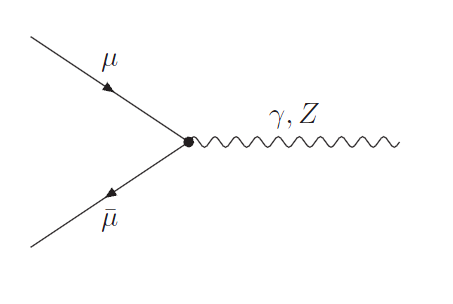
\includegraphics[width=0.5\textwidth]{visuals/002-MuonAntimuonAnihilation.png} }}%
            \subfloat[\centering $Z^0$ decay into muon-antimuon pair\cite{Jende_Kobel_Pospiech_Bilow_Pedersen_Ould-Saada_Gramstad}.]{{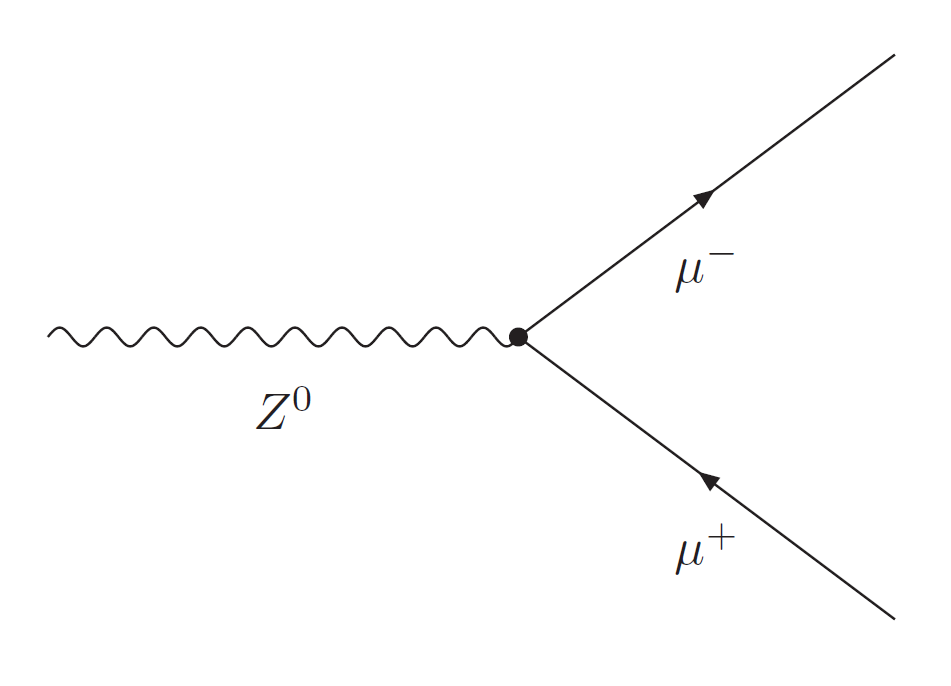
\includegraphics[width=0.5\textwidth]{visuals/001-Z_MyonAntimyon.png} }}%
            
            \caption{Feynman diagrams for the processes with Z boson and muon-antimuon pair.}
            \label{fig:001-Z_MyonAntimyon}
        \end{figure}

        When a quark from one hadron collides with an antiquark of the same flavour form another hadron there is a chance of annihilation. When the net electric charge is zero, they annihilate into virtual photon $\gamma^{*}$ or $Z$ boson\cite{ATLAS_Z_lab}. Due to a short lifetime they soon decay into a pair of leptons. This is so called \textit{Drell-Yan process}.

        \textit{Drell-Yan process} - one of the most important processes that occur in high energy hadron-hadron scattering (for example, proton-proton collisions at LHC). It happens when a quark of one hadron and an antiquark of another hadron annihilate while also creating a virtual photon or $Z$ boson which in turn decays into a pair of oppositely-charged leptons. The energy is almost entirely transformed into mass.

        \begin{figure}[H]
            \centering

            \subfloat[\centering A principal Drell-Yan process diagram\cite{ATLAS_Z_lab}.]{{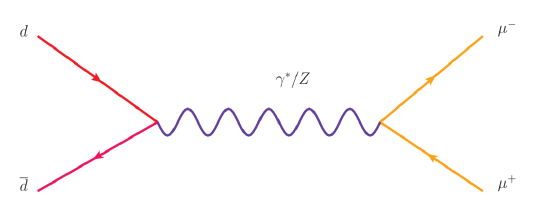
\includegraphics[width=0.5\textwidth]{visuals/003-drell-yan-simple.png} }}%
            \subfloat[\centering A more realistic Drell-Yan process diagram taking into account remnant gluon radiation processes\cite{ATLAS_Z_lab}.]{{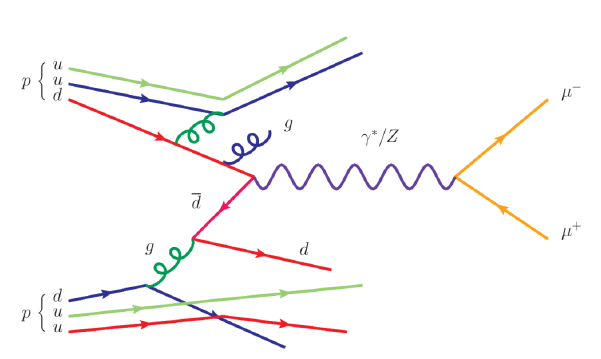
\includegraphics[width=0.5\textwidth]{visuals/004-drell-yan-real.png} }}%
            
            \caption{Feynman diagrams for Drell-Yan processes.}
            \label{fig:002-drell_yan}
        \end{figure}


        \item Processes mimicking $Z$ boson signal

        Due to its short lifetime $Z$ boson is detected by analysing the decay products. Hence, any process producing (in this case) muon-antimuon pair of a mass in the range that we would expect to find the boson would result in a fake signal. It is important to note that the signal can be produced by a bad dimuon candidate, there is no need for a physical process to happen. More on the accuracy and identification efficiency can be found under section 5.


        A few physical processes that produce muons are listed below. Notice that they are of little importance since the produced masses of muons differ vastly from the $Z$ boson decay product.

        \begin{enumerate}
            \item \textit{pion decay}
            \item \textit{W boson decay}
            \item \textit{Cosmic rays}
        \end{enumerate}


        An important phenomenon to consider when analysing $Z$ boson are "fake signals" coming from virtual photons that have high mass as they are practically indistinguishable from the $Z$ boson.

        
        \item Main graphs drawn when analysing Z boson decay into two muons. What properties are usually analysed?

        Listed below are some of the parameters extracted from a several research papers. Note that cross section of an observable has a straightforward relation to the observable itself:
        \begin{enumerate}
            \item $G_{\mu}$, $\bar{\alpha}$, $m_Z$ \cite{novikov1999theory};
            \item Muon and Z-boson momentum, pseudorapidity \cite{khodaverdian2019accuracy};
            \item Weinberg angle (indicating the strength of the $W^0$ and $B^0$ bosons mixing), pseudorapidity, $Z$ boson mass cross-section width \cite{ATLAS_Z_lab};
            \item Dimuon invariant mass $m_{\mu^{+} \mu^{-}}$ distribution, transverse momentum $p_T$ distribution \cite{Bursche:2014ltl}.
        \end{enumerate}

        From this list it is clear that the main parameters to be analysed are:
        \begin{enumerate}
            \item Pseudorapidity.
            \item Weinberg angle.
            \item $Z^0$ boson mass (same as dimuon invariant mass) distribution.
            \item Muon and Z-boson momentum.
            \item Transverse momentum $p_T$.
        \end{enumerate}


        \item Theoretical calculation of Z boson mass from two muons.


        Since $Z$ boson through Drell-Yan process decays into dimuon pair with little energy loss, we could approximate its mass to be that of the \textit{invariant mass} of muon pair.

        \textit{Invariant mass} - a variable that is constant in respect to a moving observer; for a particle with energy $E$ and momentum $\vec{p}$ it is defined as:

        \begin{equation}
            m = \frac{1}{c^2} \sqrt{E^2 - p^2c^2}
            \label{eq:001-invariant-mass}
        \end{equation}

        Invariant mass solves the relativistic problem, where both energy $E$ and momentum $\vec{p}$ measurements change depending on how fast the observer is moving. 


        

        \item LHCb detector structure, trigger, reconstruction, data validity and error.

        In this section if not explicitly specified, all information is taken (practically word-for-word) from \cite{Bursche:2014ltl} - it contains a very good description about everything.

        \begin{figure}[H]
            \centering

            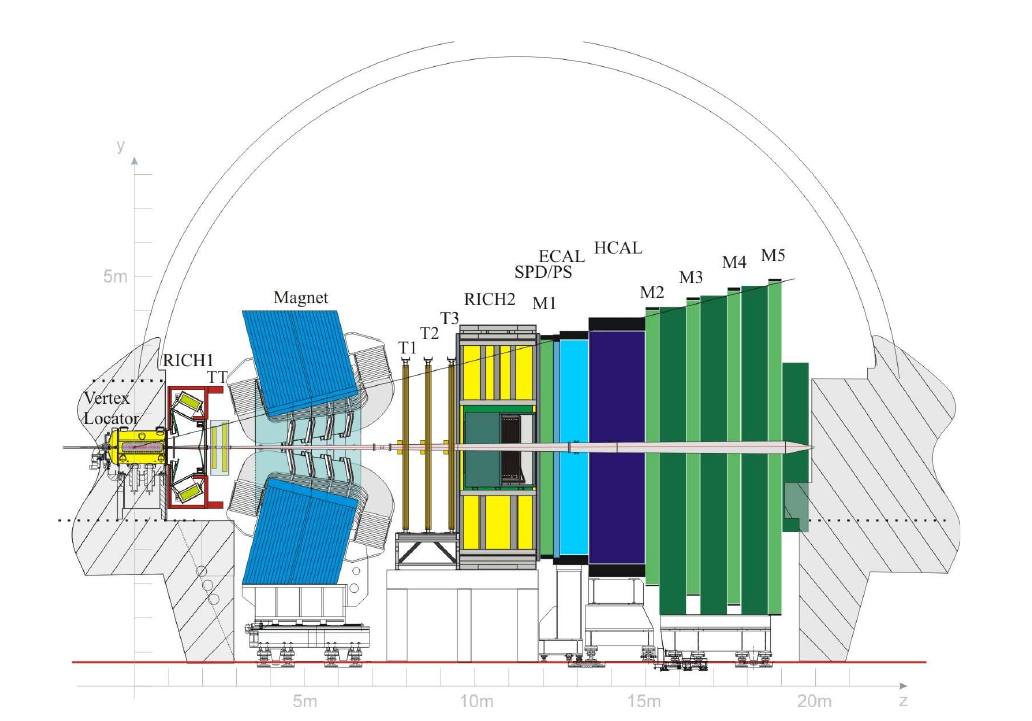
\includegraphics[width=0.7\textwidth]{visuals/005-LHCb-detector.png}
            
            \caption{LHCb detector sketch.}
            \label{fig:001-LHCb_detector}
        \end{figure}

        \begin{figure}[H]
            \centering

            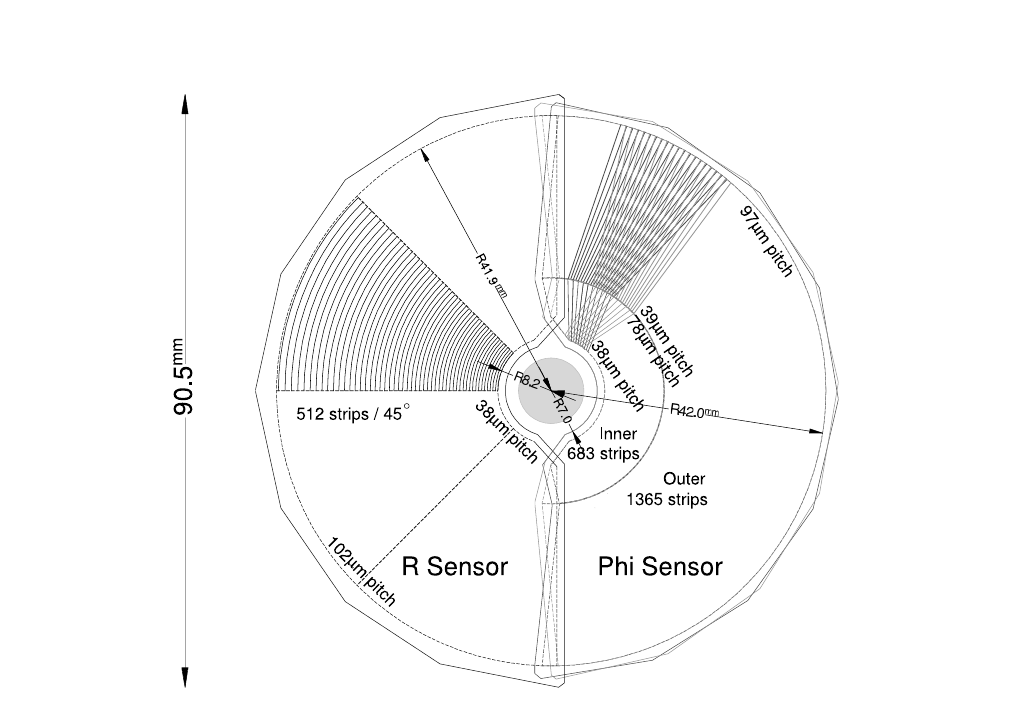
\includegraphics[width=0.7\textwidth]{visuals/006-sensors-in-VeLo.png}
            
            \caption{Sketch of the $r$ and $\phi$ sensors used in VeLo.}
            \label{fig:001-LHCb_detector}
        \end{figure}

        \underline{Cherenkov detector} - a particle passing through a material at a velocity greater than that at which light can travel through the material emits light. This is similar to the production of a sonic boom when an airplane is traveling through the air faster than sound waves can move through the air. The direction this light is emitted is on a cone with angle $\Theta_c$ about the direction in which the particle is moving, with $cos(\Theta_c) = \frac{c}{nv}$ (c = the vacuum speed of light, n - the refractive index of the medium, and v is the speed of the particle). The angle of the cone $\Theta_c$ thus is a direct measure of the particle's speed. 

        \underline{Cherenkov angle} - as in sonic booms and bow shocks, the angle of the shock cone is directly related to the velocity of the disruption. The Cherenkov angle is zero at the threshold velocity for the emission of Cherenkov radiation. The angle takes on a maximum as the particle speed approaches the speed of light. Hence, observed angles of incidence can be used to compute the direction and speed of a Cherenkov radiation-producing charge.

        \begin{figure}[H]
            \centering

            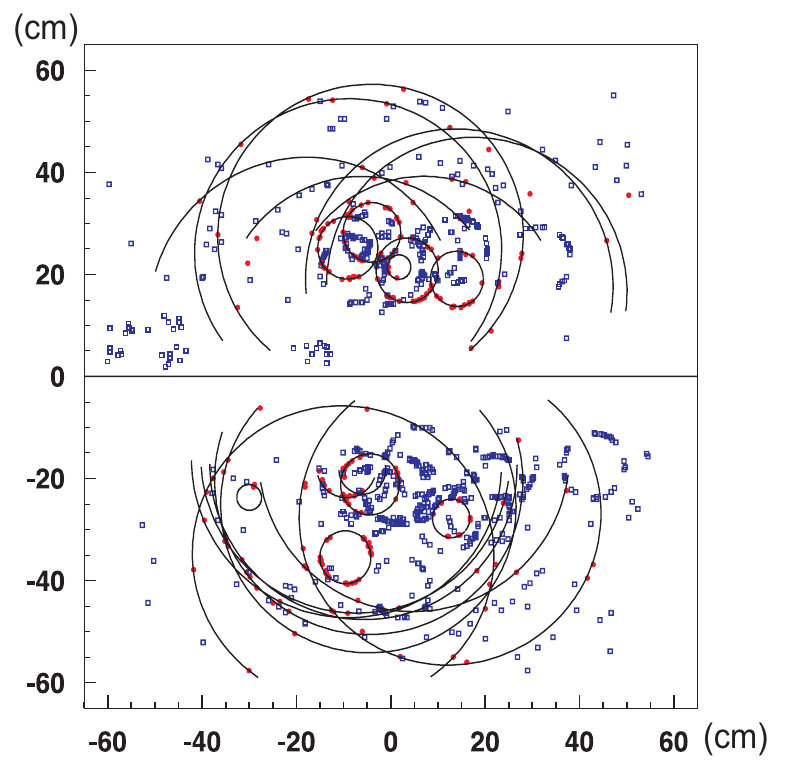
\includegraphics[width=0.7\textwidth]{visuals/007-cherenkov-simulated-RICH1.png}
            
            \caption{Simulated event as seen from RICH1\cite{Bursche:2014ltl}.}
            \label{fig:007-RICH1-simulation}
        \end{figure}

        \begin{figure}[H]
            \centering

            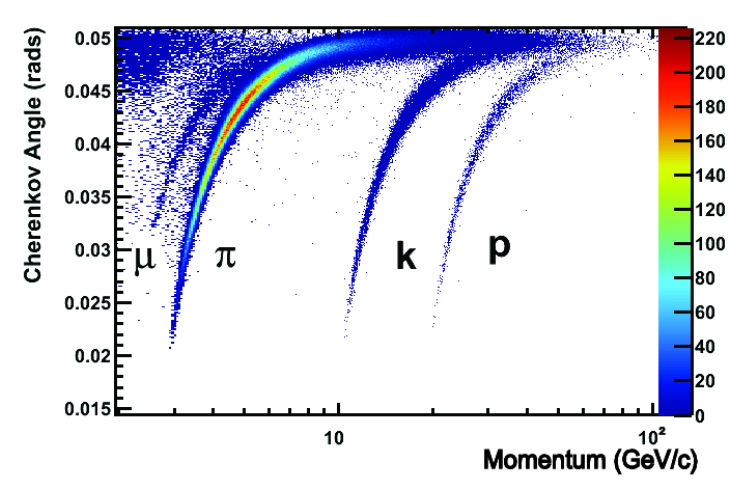
\includegraphics[width=0.7\textwidth]{visuals/008-cherenkov-angle-distribution.png}
            
            \caption{Distribution of Cherenkov angle and momentum in the \ce{C4 F10} radiator gas of RICH1\cite{Bursche:2014ltl}.}
            \label{fig:007-RICH1-simulation}
        \end{figure}



        Tracking system consists of:
        \begin{enumerate}
            \item \textbf{Vertex locator (VeLo)} - a silicon strip detector very close to the interaction point measuring the radial and azimuthal coordinates.

            \item \textbf{TT} - another silicon strip detector with two stereo layers at $5^\circ$  in front of a dipole magnet with a peak field strength of $1 T$.

            \item \textbf{T} - another tracking station after the magnet consisting of silicon strip detectors in the forward region (IT) and drift tubes are more central rapidity (OT).
        \end{enumerate}

        Track types:
        \begin{enumerate}
            \item \textbf{VeLo} - tracks that are ensured only by the VeLo. Those tracks are mainly used to find \underline{primary vertex and the decay vertices}. The magnetic field integral seen by these tracks is small and this there is \textit{no momentum estimate available}.
            
            \item \textbf{backward} - like VeLo tracks but those tracks are pointing in the backward direction.
            
            \item \textbf{upstream} - VeLo tracks extrapolated to the TT station and \textit{matched to hits in the TT station}. These tracks do see the fringe field of the magnet and this \underline{have a momentum estimate}. These tracks can in principle be reconstructed at very low momentum but practically the momentum acceptance is limited by the search windows in the algorithm to $p_T > 200 MeV$.
            
            \item \textbf{T} - tracks reconstructed in T stations only. These tracks don't see a large magnetic field inside the measured segment but together with the assumption that they originate from the PV \underline{they can get a momentum estimate assigned}. These tracks \underline{play a role as intermediate objects in the reconstruction of other tracks} and also for the understanding of the \underline{contribution of secondary particles to the photons seen in RICH2}. They are also used to \underline{veto charged particles in the neutral hadron reconstruction for jets}.

            \item \textbf{RICH1, RICH2} - two ring imaging Cherenkov detector (1 - upstream; 2 - downstream of the dipole magnet). Used to discriminate between the stable charged hadrons for the execution of the extensive flavour physics programme of LHCb. Several radiators are used in order to reach a good sensitivity in a large momentum region. There are two radiators (aerogel and \ce{C4} \ce{F10}) in RICH1 and one radiator (\ce{CF4}) in RICH2.
            
            \item \textbf{downstream} - T tracks matched to hits in the TT station. Those tracks \underline{have measurements on both sides of the dipole magnet and thus a well measured momentum}. For physics analyses they are of special importance for the reconstruction of $K^{0}_{S}$ and $\Lambda$ which often decay after the VeLo.
            
            \item \textbf{long} - tracks that do have measurements both in the VeLo and the T station. Hits in the TT station are not required for a long track and added when found compatible. \underline{If foud these hits improve momentum resolution} and recurse the probability that the long track is a random combination of hits tht does not correspond to a real particle i. e. a ghost. \underline{Long tracks are the major workhorse of the physics analyses}.
            
            \item \textbf{$\mu$ stubs} - tracks reconstructed in the \underline{muon system} only. Their major use is in the \textit{earliest trigger stage}. With the assumption that muons tracks originate from the luminous region \underline{a momentum estimate is possible}. This allows to trigger on \underline{high momentum muons and dimuons}.
            
            \item \textbf{$\mu$ TT} - muon stubs reconstructed offline that are matched to hits in the TT station. Those track are mainly used for the \underline{estimation of the efficiency} for the reconstruction of long tracks.
            
            \item \textbf{TT} - not reconstructed since the TT station has four layers with a stereo angle. Thus a particle leaving hits in all layers would have two points measured that can be reconstructed as a straight line. There is no redundancy in such a measurement and thus no $\chi^2$ and no handle to discriminate ghost tracks.
        \end{enumerate}

        The \textbf{calorimeter} system is mainly designed for the use in the \textbf{trigger} and for \textbf{particle identification}:
        \begin{enumerate}
            \item \textbf{Scintilating pad detector (SPD)} - the first layer. It consists o scintillating pads of different size made from doped polystyrene which are read for each bunch crossing using wavelength shifting fibres. It serves two purposes. In the earliest trigger stage the number of pads that see a signal is used as a \underline{measure of the total occupancy}. Events with less than 10 cells fired are selected by triggers for exclusive processes. The total multiplicity is also used to reject events at the trigger level that require a lot of CPU time in the later software triggers. \textit{Single muon trigger requires the multiplicity to be less than 600 hits and the dimuon trigger asks for less than 900 hits}. The second use of the SPD is \underline{discrimination of electron and photon candidates both at trigger level and offline}. Electrons are more likely to leave a signal in the SPD since that detector doesn't contain absorbers.
            
            \item \textbf{Preshower (PS)} - is built in a similar way as the SPD, but separated from the SPD by a 15 mm lead plate which corresponds to 2.5 electromagnetic radiation lengths. \underline{This is used to discriminate electrons and photons from hadrons}
            
            \item \textbf{Electromagnetic calorimeter (ECAL)} - is a calorimeter build in the shashlik technology. That is a structure of lead tiles interleaved by scintillator tiles which are read out by wavelength shifting fibers. It covers 25 electromagnetic radiation lengths. At very high momentum it saturates which limits the bremsstrahlung correections on electrons and significantly \textit{worsens the mass resolution} in the $Z \rightlongarrow e^{+} e^{-}$.
            
            \item \textbf{Hadronic calorimeter (HCAL)} - is not meant to reconstruct particle candidates to be used in any offline analysis. Its main purpose is to \underline{provide a trigger for full hadronic final states of the beauty hadron}. Therefore compromises have been made - especially in terms of the limited space in the cavern - leading to a calorimeter that uses 5.6 hadronic interaction lengths in only 1.6 meters.
        \end{enumerate}

        The trigger is organised in three stages:
        \begin{enumerate}
            \item \textbf{L0} - is implemented in hardware and reduces the collision rate from about 20 MHz to 1 MHz.
            \item \textbf{Hlt1} - is executed on standard CPUs.
            \item \textbf{Hlt2} - only logically separated from \textit{Hlt1}. 
        \end{enumerate}


        \item Data types used in LHCb.

        If not otherwise specified, all the information is directly taken from \textit{LHCb starterkit} article on data flow.\cite{LHCb-STARTERKIT-DATAFLOW}

        Collisions recorded by the LHCb detector go through a specific data flow designed to maximise the data-taking efficiency and data quality. This consists of several steps, each one being controlled by an ‘application’ that processes the data event-by-event, using the data from the previous step and creating the results ready for the next. These steps are as follows:

        \begin{enumerate}
            \item Data from the detector are filtered through the trigger, which consists of the $L0$, implemented in hardware, and the high level trigger ($HLT$), implemented in software. The application responsible for the software trigger is \textit{Moore}.

            \item Triggered, raw data are reconstructed to transform the detector hits into objects such as tracks and clusters. This is done by the \textit{Brunel} application. The objects are stored into an output file in a \textbf{DST} format.

            \item The reconstructed DST files are suitable for analysis, but they are not accessible to users due to computing restrictions. Data are filtered further through a set of selections called the stripping, controlled by the \textit{DaVinci} application which write out data either in the \textbf{DST} or \boldsymbol{\micro DST} format. To save disk space and to speed up access for analysts, the output files are grouped into streams which contain similar selections. By grouping all of the fully hadronic charm selections together, for example, analysts interested in that type of physics don’t waste time running over the output of the dimuon selections.
        \end{enumerate}

    A DST file is a ROOT file which contains the full event information, such as reconstructed objects and raw data. Each event typically takes around $150$ kB of disk space in the DST format. The µDST format was designed to save space by storing only the information concerning the build candidates (that is, the objects used to construct particle decays like tracks); the raw event, which takes around $50$ kB per event, is discarded.
        

    Some other file data types used in the LHCb experiment are:\cite{The-GAUSS-Framework}

    \begin{enumerate}
        \item \textbf{gen} - Generator files. Files with only the /Event/Gen tree, hence only generator information and the HepMC record. The complete hard interaction is available.

        \item \textbf{xgen} - Extended generator files. Files with the /Event/MC/MCParticles and /Event/MC/MCVertices tree in addition to /Event/Gen To produce these files only the generator phase of Gauss has been run, i.e. the content in the MCtruth tree is a copy of the generator information after hadronization. In other words quarks and strings do not appear in the MCParticles Produced by Gauss framework.

        \item \textbf{rgen} - Reduced generator files (NOT used in production yet). Files with generator information only in /Event/MC/MCParticles and /Event/MC/MCVertices tree Produced by Gauss.

        \item \textbf{sim} - Simulation files. Files resulting from the detector simulation. The conffguration of the detector (all, velo open, calo only, dddb tag) is specified in the SimulationConditions. The MCtruth tree is filled with the information from the generator for primary particles and with the secondaries produced in the detector trough transport. Hits for all detectors are also present (MCHits, MCRichHits, MCCaloHits) and additional simulation information as MCRichSegments. In case of simulations with spill-over the whole information is also available for the the spill-over slots. Produced by Gauss framework.

        \item \textbf{xsim} - Extended simulation files. Files with the whole content of a simfile in which also the full /Event/Gen is copied. Produced by Gauss framework.

        \item \textbf{digi} - Digitization files. Files containing the digitization of the simulation and the raw event as from the DAQ. They result from the Boole processing. After the Moore processing the trigger information is added. They include the MCTruth, hence the /Event/MC/Particles and MC/Vertices. If an xsim file is given as input they also include the HepMC record, this is only done upon request for some specific productions. Produced by Boole, L0App and Moore.

        \item \textbf{xdigi} - Extended digitization files. Files with the whole content of both sim and digi processing. Produced by Boole, L0App and Moore.

        \item \textbf{raw} - Raw files. The raw events as produced at the Pit by the DAQ. Not used for MC.

        \item \textbf{dst} - Dst files. Files resulting from the reconstruction of real data and of MC samples. For MC they have the same identical information as that of the reconstruction run on them but also normally include the MC truth, hence the /Event/Gen and the /Event/MC/Particles and Vertices, and the association to them from high level reconstructed quantites. When Turbo is run the output of the Turbo lines is added. When Stripping is run the output of the stripping lines is added, but the RAW event is dropped. Produced by Brunel, Tesla or DaVinci. Normally production save the DST output produced by DaVinci.

        \item \textbf{ldst} - DST files with linkers. This format only applies to simulation samples: the Boole linkers from digits to MCParticles are included to allow MC association when (re-)running Moore or Brunel in addition to the DST content (that is specified above depending on the application producing the output). Produced by Brunel, Tesla or DaVinci.

        \item \textbf{xdst} - Extented DST files. This format only applies to simulation samples: the whole content of the input XDIGI (hence also SIM/XSIM) is included in addition to the DST content (that is specified above depending on the application producing the output). Produced by Brunel, Tesla or DaVinci.

        \item \textbf{microDst} - Micro DST files. Dst files with only the reconstructed information relative to the reconstructed quanties of a stripping line. In the case of simulated samples it also include the MC information associated (via the chosen associator) to these reconstructed quantities. It also contains the MCtruth of the signal for all events (at the moment only for Run2 MC). When Turbo is run it will also includes the turbo lines candidates and associated MC truth (under deployement). When the stripping is run in Flagged mode (standard productions) all events are saved, while in filtering mode only those that satosfy the filtering.

        \item \textit{other} - The data type that are a combination of \textbf{XXX.FileType}, with \textbf{FileType = dst, xdst, ...} and with \textbf{XXX = AllStream, MCFilter, etc.} indicate the subset of events that they contain.
    \end{enumerate}

    \begin{figure}[H]
        \centering

        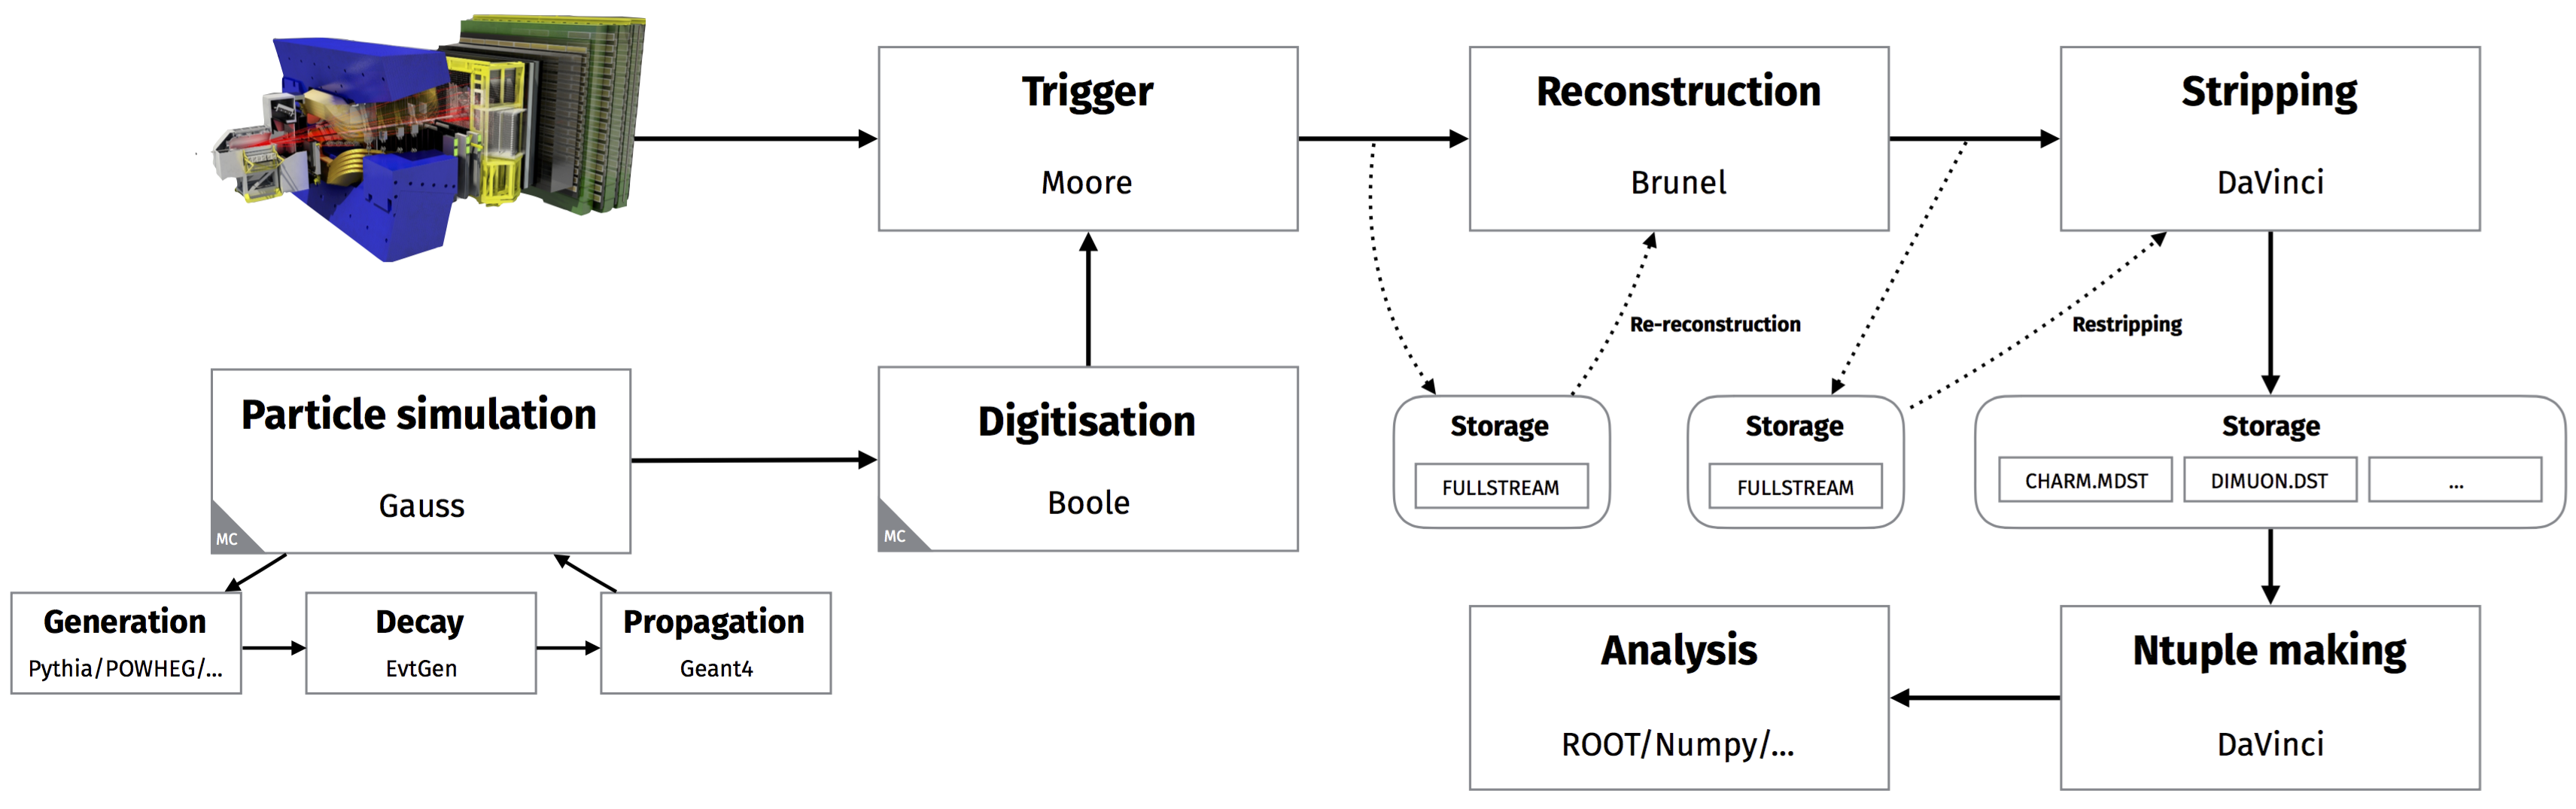
\includegraphics[width=\textwidth]{visuals/009-lhcb_data_flow.png}
        
        \caption{Data flow and the associated applications when LHCb experiment is simulated\cite{LHCb-STARTERKIT-DATAFLOW}. Note that only the first two steps are different from real-life scenario (\textit{Particle Simulation} and \textit{Digitisation}).}
        \label{fig:009-RICH1-simulation}
    \end{figure}

    
        
    \end{enumerate}


\section{Results}
    
\singlespacing
	
	%\phantomsection
	
\bibliographystyle{VUstyle}
\bibliography{mybib}
	
\end{document}
